\chapter[Experimentación]{Experimentación}\label{ch:experimetal-all}



% rand	Uniformly distributed random numbers
% randn	Normally distributed random numbers
% randi	Uniformly distributed pseudorandom integers
% randperm	Random permutation




% B = randi([1 17],20,100);


% B = randi(  [1 17], 20   , round( rand(1)*100 )   );



% save LALA B -ascii

% xlswrite('archivo.xls', datos obtenidos,'datos','A1:C2');


% La función "diary" nos permite salvar, en un fichero de texto, lo que aparezca por pantalla. Por ejemplo, el siguiente código:

% diary('diario1.txt')
% x = 3
% A = 10000;
% diary off






% Al cargar los datos desde Matlab, nos estaría creando una estructura. Para acceder a los datos y al texto, podríamos hacer:

% A = importdata('data.txt')
% B = A.data
% t1 = cell2mat(A.textdata)
% clear A



{
% Los objetivos no estan diferenciados entre generales y especıficos.
% Se presentan procesos que validan el trabajo comparando con otros metodos del estado del arte. 
% Se presenta una validacion deparametros,y todas las dimensiones que fueron planteadas son exploradas en profundidad.
% Se detalla y explica la recoleccion (de aplicar) y analisis de da- tos y resultados.
% Se distinguen los resultados segun las variables investigadas, y se examinan en virtud de lo explicado en el marco teorico.
%Se interpretan con claridad (es decir, se consideran distintos factores y anteceden- tes descritos hasta el momento) los resultados obtenidos.
}

Lo que se busca es un modelo de accesos de navegación secuencial creado por un algoritmo de compresión, Lempel Ziv,  para usarlo como un modelo  predicción. Se usará para buscar resultados sobre secuencias finitas discretas de \emph{webaccess logs}. Al momento de generar el árbol este creará una representación \emph{trie} de un diccionario de símbolos, se utilizará para realizar predicciones en secuencias discretas con distintos largos.

En base a lo anterior y teniendo en funcionamiento el algoritmo para crear un modelo de predicción, se integrará con el servidor de \emph{Machine Learning, PredictionIO} que ya se ha explicado anteriormente. Usaremos la misma \texttt{API }que ofrece la librería para poder realizar las evaluaciones de nuestras métricas, dado el dominio de nuestro problema la métrica a usar será \emph{Accuracy} (Exactitud) frente a distintas porciones de datos. Con el conjunto de datos que tenemos haremos variadas pruebas para ver métricas como Accuracy, usaremos \emph{cross validation} en distintos escenarios que nos permitirán tener información relevante de comportamiento de nuestro modelo propuesto en escenarios ideales como en escenarios reales.

%- Cross validation: This method is generally applied in machine-learning evaluation [14]. In our experiments, we performed a K-fold cross validation with k = 10. In this way, our dataset is 10 times split into 10 different sets of learning (90 
% of the total dataset) and testing (10 % of the total data).
%-Learning the model: We accomplished the learning step using different learning algorithms depending on

%%%%% Gueniche_Fournier-Viger_Raman_Tseng
%Tree is a type of prefix tree (aka trie). It contains all training sequences. Each tree node represents an item and each training sequence is represented by a path starting from the tree root and ending by an inner node or a leaf. Just like a prefix tree, the prediction tree is a compact representation of the training sequences. Sequences sharing a common prefix share a common path in the tree. The Lookup Table is an associative array which allows to locate any training sequences in the prediction tree with a constant access time. Finally the Inverted Index is a set of bit vectors that indicates for each item i from the alphabet Z, the set of sequences containing i.



\section{Nuestro modelo de predicción ML-LDC}\label{sec:nuestromodelopredict-mlldc}


%%%%%%% \cite{Moghaddam2009}

%The techniques that rely on sequential patterns such as Markov models and sequential association rules mining contain more precise information about users’ navigation behavior. 


%There is an arc from node A to B if and only if at some point in time a client accessed to B within w accesses after A, where w is the lookahead window size. The weight of the arc is the ratio of the number of accesses to B within a window after A to the number of accesses to A itself. 

Basados en un servidor de \emph{Machine Learning}, hemos desarrollado un motor de predicción con un algoritmo basado en \emph{Lempel} \& \emph{Ziv} \cite{ZivLempel1977}. Cada sesión es representada por un nodo y sus hijos. Sea la sesión \begin{equation}
Input = \{ A,A,A,B,A,B,B,B,B,B,A,A,B,C,C,D,D,C,B,A,A,A,A \}
\end{equation} la cual representaremos con nuestro modelo de predicción



\begin{figure}[h] 
	\centering
	\begin{forest} 
	[ $\epsilon$
		[A
			[AA
				[AAA]	
			]
			[AB
				[ABC]
			]
		]
		[B
			[BA]
			[BB
				[BBA]
			]
		]
		[C]
		[D
			[DC]
		]
	]
	\end{forest}
	\caption{Ejemplo de Árbol de Predicción basado en \texttt{LZ78}.}
	\label{fig:lztrie1}
\end{figure}

Dado nuestro modelo de predicción podemos determinar que nuestra salida resultante será:

\begin{equation}
Output = \{ A,AA,B,AB,BB,BBA,ABC,C,D,DC,BA,AAA \}
\end{equation}


Acotamos los siguientes casos en que nuestro Modelo de predicción funcionará:


\begin{enumerate}
	\item \textbf{Nodos Intermedios probabilidad Equivalente}
	
	Dada la $P( x | A\epsilon  )$, siendo $x$ la probabilidad de encontrar el siguiente símbolo. Este caso nos muestra que tenemos dos secuencias posibles $\{A,AB\}$, por lo cual podemos hacer la función $arg\ max(AA,AB)$ ó calcular una función $random(AA,AB)$, al ser un caso con solamente dos posibilidades tenemos solo un $50\%$ de éxito.
	
	
	\item \textbf{Nodos intermedios con un nodo hijo }
	
	Dada la $P( x | AB  )  = ABC$, ya que  el nodo $C$, es el único hijo por tanto tiene toda la certeza de ser la predicción acorde al árbol de entrenamiento.
		
		
		
	\item \textbf{Nodo hoja y vuelta a la raíz}	
	
	Este caso es uno de los más sencillos ya que nuestro modelo al no tener más secuencias para poder hacer las operaciones, se proyectará el árbol para todos los posibles accesos dentro de nuestro alfabeto. Para el caso $\Sigma = \{A,B,C,D \} $ y la probabilidad para cada acceso representado por símbolos es de $25\%$.
	
	
	Dada la probabilidad $P( x ) $ al momento de retornar a la raíz, la siguiente secuencia es absorbida por $\epsilon$.
	

\end{enumerate}







\section{Ambientes experimental}

Para los ambientes experimentales se han dispuestos dos máquinas para realizar las pruebas. 

\subsubsection{Máquinas}
	\begin{itemize}
		\menorEspacioItemize
		\item Procesador 2,8 GHz Intel Core i7, 16 GB de Memoria RAM y Sistema Operativo OSX
		\item Procesadores Intel Xeon E5-2670 v2 (Ivy Bridge) de alta frecuencia 32 vCPU, 244 GB de Memoria RAM y Sistema Operativo Ubuntu 14.14 
	\end{itemize}
	
Para el proceso de desarrollo con \emph{IntelliJ} y un conjunto de datos menores a 500 sesiones se usará la máquina con 16GB y para experimentos con sesiones mayores a 10000 sesiones de usuarios se usará la máquina 240GB.	
	

\subsubsection{Software utilizado}

	\begin{itemize}
		\menorEspacioItemize
	
		\item C++11
		\item Java  1.8
		\item Java(TM) SE Runtime Environment (build 1.8)
		\item Java HotSpot(TM) 64-Bit Server VM (build $25.51-b03$, mixed mode)
		\item Scala code runner version 2.11.7 -- Copyright 2002-2013, LAMP/EPFL
		\item SBT 0.13.9 
		\item Python 2.7.10
		\item GNU bash 3.2.57 $(x86_64-apple-darwin15)$
		\item Prediction.IO 0.9.4
		\item Elasticsearch 1.4.4	
		\item Apache Spark-1.4.1
		\item Hbase 1.0.0
		\item Zookeeper 
	\end{itemize}



% Selección de la métrica
% https://docs.prediction.io/evaluation/metricchoose/
% Explicación de evaluación
% https://docs.prediction.io/templates/recommendation/evaluation/#evaluation-data-generation




El motor de predicción es \emph{PredictionIO}, como se ha señalado anteriormente  es un entorno de desarrollo para desplegar servidores con algoritmos de \emph{Machine Learning} como  \emph{Decission Tree, K-Means, RNN} y todos los algoritmos ofrecidos por la librería de \emph{Apache Spark} y \emph{MLib}. Para desarrollar un motor que se acople con \emph{PredictionIO} se deberá seguir el patrón \emph{DASE}\ref{dase-algoritmo} y crear un modelo con persistencia en memoria que nos permita un acceso rápido a las predicciones por consulta.


Usaremos \emph{SBT} para gestionar todas las librerías que se requieran como dependencia. Inherentemente usaremos \emph{Java}, ya que el lenguaje \emph{Scala} corre sobre la \emph{Java Virtual Machine}. \emph{Prediction.IO} no solo ocupa \emph{Scala}, adicionalmente provee el uso de {Apache Spark} con sus librerías de \emph{MLIB} (\emph{Machine Learning Library}), \emph{Zookeeper}, \emph{Hbase} (Hadoop) y \emph{Elasticsearch}. Hemos utilizado \emph{Python} para realizar un cliente por línea de comando en el cual poder hacer pruebas y adicionalmente incluir un cliente que realice la carga de eventos desde nuestro set de datos experimental. Para mayor referencia de los clientes ver los códigos en anexos.





% Es una métrica que captura una porición correcta de toda la data a probar. 
% Una manera de modelar esto es para cada consulta que hacemos al predictor, damos un score de 1 y 0, luego podemos tomar el promedio de este score.

% PredictionIO sobre métricas


% PredictionIO has a [[AverageMetric]] helper class which provides this feature. This class takes 4 type parameters, [[EvalInfo]], [[Query]], [[PredictedResult]], and [[ActualResult]], these types can be found from the engine's signature. Line 5 below is the custom calculation.

%Precision is a metric for binary classifier capturing the portion of correction prediction among all positive predictions. We don't care about the cases where the QPA-tuple gives a negative prediction. (Recall that a binary classifier only provide two output values: positive and negative.) The following table illustrates all four cases:

%Calculating the precision metric is a slightly more involved procedure than calculating the accuracy metric as we have to specially handle the don't care negative cases.

%x PredictionIO provides a helper class OptionAverageMetric allows user to specify don't care values as None. It only aggregates the non-None values. Lines 3 to 4 is the method signature of calcuate method. The key difference is that the return value is a Option[Double], in contrast to Double for AverageMetric. This class only computes the average of Some(.) results. Lines 5 to 13 are the actual logic. The first if factors out the positively predicted case, and the computation is simliar to the accuracy metric. The negatively predicted case are the don't cares, which we return None.

% \subsection{Experimento comparativo con Frequent Sequency Pattern}


%\subsection{Decission Tree}
%\subsection{Asociation Rulz}





\section{Datos experimentales}
	% Cita a Rkonow Claude & Navarro

Se usarán las secuencias disponibles de \emph{webaccess logs} pública del sitio \emph{MSNBC}. El conjunto de datos corresponde a los registros del servidor {IIS} (Internet Information Services) de \emph{msnbc.com}, de un día completo de la fecha  28 de Septiembre de 1999. 
Contiene secuencias de acceso \emph{web} de 989,818 usuarios con un promedio de 5,7 categorías \emph{web} visitas por secuencia, el tamaño del alfabeto de este conjunto de datos es, $\sigma \ = 17$.




Utilizaremos un simple programa\footnote{Este programa se encuentra junto en el anexo de la memoria} en \texttt{C++ }para filtrar las sesiones de los usuarios, creando nuevos set de datos y transformarlos a símbolos, caracteres en mayúscula, por ejemplo en la figura \ref{fig:sesiones-ds-msbc-num}  y Figura \ref{fig:sesiones-ds-basicos} se encuentra una muestra de las entradas que disponemos para trabajar. El set de datos de la Figura \ref{fig:sesiones-ds-basicos}, es el formato que utilizaremos para generar el modelo.


\begin{figure}[t] 
	\centering
	\begin{lstlisting}[frame=single,basicstyle=\ttfamily\tiny,]
	1 1 
	2 
	3 2 2 4 2 2 2 3 3 
	5 
	1 
	6 
	1 1 
	6 
	6 7 7 7 6 6 8 8 8 8 
	6 9 4 4 4 10 3 10 5 10 4 4 4 
	\end{lstlisting}	
	\caption{Secuencia de datos con indices numéricos del set de datos MSNBC}
	\label{fig:sesiones-ds-msbc-num}
\end{figure}




\begin{figure}[t] 
	\centering
	\begin{lstlisting}[frame=single,basicstyle=\ttfamily\tiny,]
	% Different categories found in input file:
	
	frontpage news tech local opinion on-air misc weather msn-news health living business msn-sports sports summary bbs travel
	
	% Sequences:
	A A 
	B 
	C B B D B B B C C 
	A A 
	F 
	F G G G F F H H H H 
	F I D D D J C J E J D D D 
	A A A K A A A 
	L L 
	A A 
	H H H H H H 
	\end{lstlisting}
	\caption{Ejemplo de sesiones de usuarios en símbolos dataset \emph{MSNBC}.}
	\label{fig:sesiones-ds-basicos}
\end{figure}






Ejemplo de sub-dataset creados
\begin{itemize}
	\setlength{\itemsep}{0.9pt}
	\setlength{\parskip}{0pt}
	\setlength{\parsep}{0pt}
	\item Secuencias de \emph{webaccess} con sesiones con umbral mínimo.
	\item Secuencias de \emph{webaccess} con sesiones de largo equivalente.
	\item Secuencias de \emph{webaccess} con sesiones de más de 100 secciones web visitadas.
	\item Secuencias de \emph{webaccess} con sesiones acotadas superiormente.
\end{itemize}


Trabajaremos con aproximadamente $1.000.000$ de registros los cuales hemos realizados distintos subconjuntos para hacer una validación cruzada:

\begin{itemize}
	\setlength{\itemsep}{1pt}
	\setlength{\parskip}{0pt}
	\setlength{\parsep}{0pt}
	\item 10 Sesiones de usuarios
	\item 100 Sesiones de usuarios
	\item 1.000 Sesiones de usuarios
	\item 10.000 Sesiones de usuarios
	\item 50.000 Sesiones de usuarios
	\item 100.000 Sesiones de usuarios
	\item 500.000 Sesiones de usuarios
	\item 1.000.000 Sesiones de usuarios
\end{itemize}


Es importante señalar que la división de nuestro set de datos es debido a que no conocemos la naturaleza de los mismos, pero con nuestro modelo podemos estudiarlos para ir detectando patrones que puedan ser claves para medir el rendimiento en función a los criterios de volumen de datos versus \emph{Accurracy}.






\begin{table}[]
	\centering
	\label{table-list-symbol}
	\begin{tabular}{cl}
		Page       & Symbol \\ \cline{1-2}
		frontpage  & A      \\
		news       & B      \\
		tech       & C      \\
		local      & D      \\
		opinion    & E      \\
		on-air     & F      \\
		misc       & G      \\
		weather    & H      \\
		msn-news   & I      \\
		health     & J      \\
		living     & K      \\
		business   & L      \\
		msn-sports & M      \\
		sports     & N      \\
		summary    & O      \\
		bbs        & P      \\
		travel     & Q      \\ 
	\end{tabular}
	\caption{Equivalencia secciones msnbc y símbolo representativo.}
\end{table}




\section{Experimentos}



Dentro de nuestro experimentos para probar la exactitud de nuestro modelo podemos demostrar que al tener una menor cantidad de secciones visitadas, la probabilidad de no acertar crece considerablemente.


Sea la siguiente sesión de un usuario 
$\{A , B , A  \}  $ para un alfabeto $\Sigma=\{A,B,C,D,E,F,G,H,I,J,K,L,M,N,O,P,Q \} $





\begin{figure}[h] 
	\centering
	 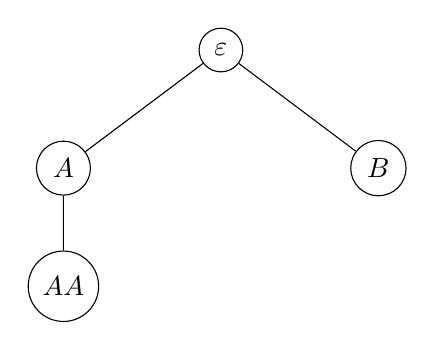
\begin{tikzpicture}[level/.style={sibling distance=40mm/#1}]
		\node [circle,draw] (epsilon){$\varepsilon$}
		child { node [circle,draw] (A) {$A$} 
			child { node[circle,draw](AA){$AA$}  }
		}
		child {node [circle,draw] (B) {$B$} }
		;
		
		\end{tikzpicture}
	\caption{Ejemplo de Modelo de predicción basado en un \emph{trie} con \texttt{LZ78}.}
	\label{fig:sim}
\end{figure}



Podemos ver que a menor cantidad de símbolos en la sesión generan un árbol de menor altura y menos nodos, cada nodo como se ha señalado en el capitulo 4 representa un visita a una sección en particular de la web de \emph{MSNBC}. Cuando un \emph{webaccess} posee  pocas secciones o páginas visitadas, la proyección de probabilidades de los posibles símbolos en el alfabeto hace que la probabilidad del siguiente acceso sea equiprobable dentro del los símbolos de nuestro diccionario, de lo anterior convergemos en que mayor es el entrenamiento mejor será la predicción.

Dado el evento $x$  a predecir que pertenece a una secuencia discreta, la probabilidad de $P( x| AB  ) = A $, es el resultado de esta sesión de entrenamiento, pero la probabilidad $P(x | AAB) $, es desconocida.  Si extendemos los símbolos de este nodo cada nodo hijo tendría un probabilidad de $ \dfrac{1}{\Sigma} = \dfrac{1}{17} = 0.0588 $ o bien sería  $\dfrac{1}{ |\sigma| }$, siendo $|\sigma|$ el total de símbolos que se encuentran en el alfabeto. 

Para corroborar este comportamiento haremos distintos experimentos en distintos volúmenes de datos, usaremos una validación cruzada para medir el \emph{Accuracy}, la cual será nuestra métrica a utilizar.

Con esto demostraremos que secuencias con menores cantidad de símbolos generar un tipo de ruido a la métrica  que afecta en su a nuestra exactitud esperada, cuando hacemos nuevos ciclos de evaluaciones sobre el mayor orden, por otra parte veremos como con una menor cantidad de sesiones de entrenamiento podemos lograr un \emph{Accuracy} bastante optimista.



\vspace{1cm}
\begin{enumerate}
	% Idea de experimento con disminución del tamaño del alfabeto
	\item\label{exp1} \textbf{Experimento con sesiones de usuarios con datos generados de forma sintética}
	
	Creamos un set de datos en el cual pudiésemos esperar valores conocidos. Además acotamos a un diccionario de solo tres elementos, el Accurracy obtenido es:
	
	
	
	\begin{figure}[h] 
		\centering
			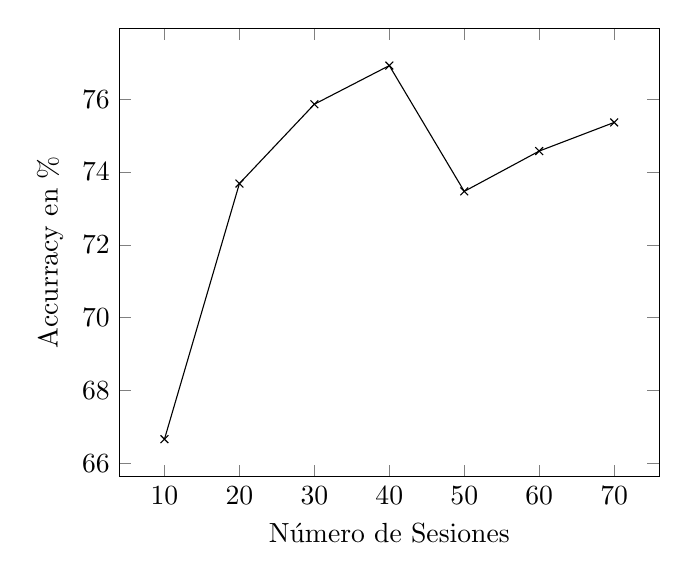
\begin{tikzpicture}
			\begin{axis}[
			xlabel= Número de Sesiones,
			ylabel=Accurracy en \% ]
			\addplot[color=black,mark=x] coordinates {
				(10, 66.6666666666666)
				(20, 73.6842105263157)
				(30, 75.8620689655172)
				(40, 76.9230769230769)
				(50, 73.469387755102)
				(60, 74.5762711864406)
				(70, 75.3623188405797)
			};
			\end{axis}
			\end{tikzpicture}	
		\caption{Experimento con set de datos sintéticos.}
		\label{fig:graph-exp1}
	\end{figure}
	

	
 
	
	En el gráfico \ref{fig:graph-exp1} usamos como mínimo 10 sesiones de las 80 de disponibles que se usaron par este experimento. Dado a que en este caso la cantidad de sesiones es bien reducida y cada símbolo posee una gran frecuencia existe mayor redundancia de datos y nuestro modelo se comporta como espera que lo haga un algoritmo de compresión de datos. Entre mayor es la cantidad de símbolos iguales
	que van entrenando al \emph{trie}, hay una aglomeración de frecuencia en ciertos nodos, pero estos son minimizados por los niveles que genera al momento de la construcción del árbol.
	
	La tasa de frecuencia de un símbolo converge a predicciones de secuencias evaluadas que caen en el nodo con mejor probabilidad dado $\epsilon$ (raíz del \emph{trie}).
	



	
   \begin{figure}[h] 
	   \centering
	   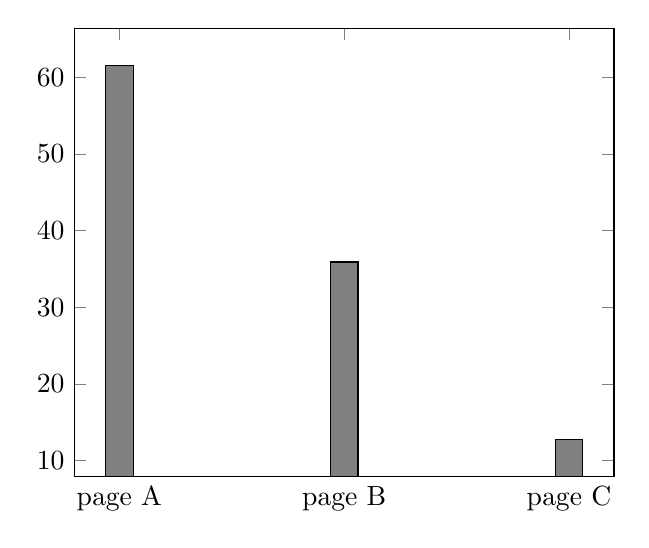
\begin{tikzpicture}
	   \begin{axis}[
	   symbolic x coords={ page A, page B, page C},
	   xtick=data
	   ]
	   \addplot[ybar,fill=gray] coordinates {
	   	(page A,   61.5)
	   	(page B,  35.9)
	   	(page C,   12.8)
	   };
	   \end{axis}
	   \end{tikzpicture}
		\caption{Distribución de símbolos para set de datos sintéticos.}
		\label{fig:bar-chart-data-sintetica}
	\end{figure}


	\begin{table}[]
		\centering
		\label{tabla-exp-1}
		\begin{tabular}{ccccc}
			\textbf{pruebas}     & \textbf{entrenamiento} & \textbf{accuracy}    & \textbf{nodos}       & \textbf{niveles}     \\
			10                   & 90                     & 0,753623188405797    & 10                   & 5                    \\
			20                   & 80                     & 0,745762711864406    & 10                   & 5                    \\
			30                   & 70                     & 0,73469387755102     & 10                   & 5                    \\
			40                   & 60                     & 0,769230769230769    & 10                   & 5                    \\
			50                   & 50                     & 0,758620689655172    & 10                   & 5                    \\
			60                   & 40                     & 0,736842105263157    & 10                   & 5                    \\
			70                   & 30                     & 0,666666666666666    & 10                   & 5                    \\
			&                        &                      &                      &                      \\
			\multicolumn{1}{l}{} & \multicolumn{1}{l}{}   & \multicolumn{1}{l}{} & \multicolumn{1}{l}{} & \multicolumn{1}{l}{}
		\end{tabular}
		\caption{ Resumen de datos experimento 1}
	\end{table}






	\begin{table}[] 	\label{tabl-exp-1-frec}
		\centering
		\resizebox{0.9\textwidth}{!}{% <------ Don't forget this %
	
		\begin{tabular}{lccccccccccccccccc}
			\textbf{símbolo}    & A  & B  & C  & D  & E & F  & G  & H  & I  & J  & K & L  & M  & N  & O & P & Q \\
			\textbf{frecuencia} & 400 & 280 & 100 & 0 & 0 & 0 & 0 & 0 & 0 & 0 & 0 & 0 & 0 & 0 & 0 & 0 & 0
		\end{tabular}
		
	}
		\caption{Tabla de frecuencia experimento 1}
	\end{table}



	Tal como se puede ver en el gráfico \ref{fig:bar-chart-data-sintetica} existe un gran probabilidad de que dado una secuencia de accesos después de $\epsilon$ la próxima sección a acceder sea la página A.
	Esto es adicionalmente es consistente a el tipo de set de datos que hemos ocupado ya que con esto podemos delimitar a que nuestro modelo al tener símbolos bastante frecuente no crea un trie desbalanceado, para este caso solo acota constantemente a un altura de 5 niveles y una variación mínima entre la exactitud, que posee el entrenamiento versus set de evaluaciones, incluso podemos solo podemos usar un entrenamiento de por lo menos 30 sesiones para predecir 50 sesiones con un Accurracy con un margen de error máximo de $10\%$ en el peor de los casos. 
	Lo anterior si lo comparamos con un evento aleatorio como resultado nos daría que nuestro modelo es bastante mejor que una predicción aleatoria, es decir $ 66.7\%  \geq 33\%$, siendo esta una comparativa optimista de que al menos nuestro modelo dado un set de datos artificial.
	



	
	
	
	\newpage
	\item \label{exp2} \textbf{Sesiones con menor redundancia y  largo variable }
		
	Validaremos ahora el comportamiento de nuestro modelo con datos reales con secuencias discretas distribuidas no uniformemente.
	
	
	
	\begin{figure}[h] 
		\centering
				\resizebox{0.6\textwidth}{!}{% <------ Don't forget this %
			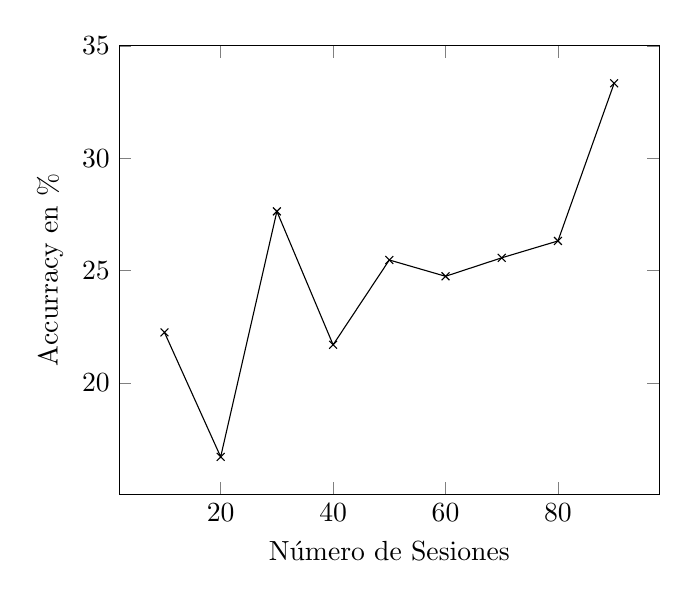
\begin{tikzpicture}
			\begin{axis}[
			xlabel= Número de Sesiones,
			ylabel=Accurracy en \% ]
			\addplot[color=black,mark=x] coordinates {
				(10, 22.2471910112359)
				(20, 16.7088607594936)
				(30, 27.6328502415459)
				(40, 21.6949152542372)
				(50, 25.469387755102)
				(60, 24.7435897435897)
				(70, 25.5665024630541)
				(80, 26.3157894736842)
				(90, 33.3333333333333)
			};
			\end{axis}
			\end{tikzpicture}
		}
		\caption{Experimento con secuencias de largo variable}
		\label{fig:experimento2}
	\end{figure}
	

	\begin{table}[h]
		\centering
		\label{tabla-exp-1}
		\begin{tabular}{ccccc}
			\textbf{pruebas}     & \textbf{entrenamiento} & \textbf{accuracy}    & \textbf{nodos}       & \textbf{niveles}     \\
			10                   & 90                     & 0,222471910112359    & 10                   & 5                    \\
			20                   & 80                     & 0,167088607594936    & 10                   & 5                    \\
			30                   & 70                     & 0,27632850241546     & 10                   & 5                    \\
			40                   & 60                     & 0,21694915254237     & 10                   & 5                    \\
			50                   & 50                     & 0,25469387755102     & 10                   & 5                    \\
			60                   & 40                     & 0,24743589743590   	 & 10                   & 5                    \\
			70                   & 30                     & 0,255665024630541    & 10                   & 5                    \\
			80                   & 20                     & 0,263157894736842    & 10                   & 5                    \\
			90                   & 10                     & 0,333333333333333    & 10                   & 5                    \\
			&                        &                      &                      &                      \\
			\multicolumn{1}{l}{} & \multicolumn{1}{l}{}   & \multicolumn{1}{l}{} & \multicolumn{1}{l}{} & \multicolumn{1}{l}{}
		\end{tabular}
		\caption{ Resumen de datos experimento 1}
	\end{table}



	\begin{table}[h] 	\label{tabl-exp-1-frec}
		\centering
		\resizebox{0.9\textwidth}{!}{% <------ Don't forget this %
	
		\begin{tabular}{lccccccccccccccccc}
			\textbf{símbolo}    & A  & B  & C  & D  & E & F  & G  & H  & I  & J  & K & L  & M  & N  & O & P & Q \\
			\textbf{frecuencia} & 64 & 19 & 18 & 29 & 4 & 36 & 20 & 65 & 20 & 11 & 4 & 15 & 42 & 31 & 2 & 0 & 0
		\end{tabular}
		
	}
		\caption{Tabla de frecuencia experimento 1}
	\end{table}


			
	En este caso si existe una menor redundancia a diferencia del experimento \ref{exp1} lo que produce que el modelo $M$ tenga un bajo rendimiento, aún así dada sigue siendo en el mejor de los casos seis veces mejor que la probabilidad aleatoria de predecir. En este experimento usamos un $|\sigma| =15$, por ende tenemos que dado nuestro modelo,
	\begin{equation}\label{expResult2}
		M( x | \mbox{90\% train}  ) = 33 \% \geq M( x | \mbox{random}  ) = 6.66 ,\% 
	\end{equation} como hemos visto en el experimento \ref{exp1} nuestro modelo sigue siendo válido en un escenario en que los datos se dispersan considerablemente. 
	Adicionalmente en este tipo de caso existe un comportamiento de nuestro modelo en el cual hace el mejor esfuerzo por mantener la \emph{compresibilidad} de los datos mayor o igual a la \emph{predictibilidad} del mismo, peor al tener mayor dispersión la altura para una cantidad similar de sesiones en \ref{exp1} sigue siendo $5$. Pero la cantidad de nodos sufre un gran incremento, podemos verlo en \ref{fig:exp-largo-variable-inf}
	
	
	
	\begin{figure}[h] 
		\centering
		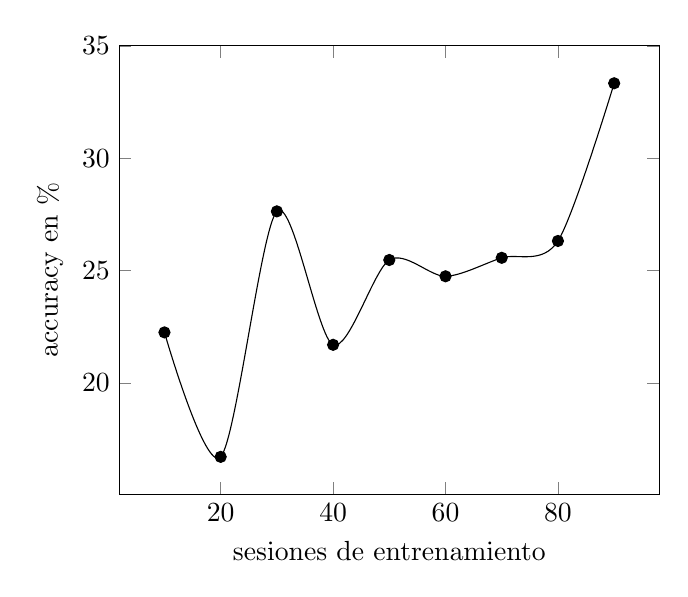
\begin{tikzpicture}
		\begin{axis}[
		xlabel=$\mbox{sesiones de entrenamiento}$,
		ylabel=$\mbox{accuracy en \%}$]
		\addplot[smooth,mark=*,black] plot coordinates {
			(10, 22.2471910112359)
			(20, 16.7088607594936)
			(30, 27.6328502415459)
			(40, 21.6949152542372)
			(50, 25.469387755102)
			(60, 24.7435897435897)
			(70, 25.5665024630541)
			(80, 26.3157894736842)
			(90, 33.3333333333333)
		};
		\end{axis}
		\end{tikzpicture}	
		
		\caption{Experimento con secuencias de largo variable inferiores y 100 sesiones}
		\label{fig:exp-largo-variable-inf}
	\end{figure}
	
	
	



	Acorde al gráfico \ref{fig:exp-largo-variable-inf} podemos señalar que al haber un incremento en la dispersión de datos y menor redundancia, el crecimiento de nuestro árbol será horizontal, ya que para tanto como hemos en este experimento y en (\label{expResult2}), la altura del nodo no tiene una relación directa a la redundancia ó dispersión, pero si a la cantidad de sesiones evaluadas. 
	
	Además, al mayor esfuerzo que hace el predictor por lograr mejores resultados se construyen mas nodos, por lo que el modelo LDC, deja de comprimir por satisfacer las condiciones de predictibilidad necesarias para seguir siendo válido.

	
	Iteramos una nueva evaluación con las mismas condiciones pero subiendo el volumen de datos de 100 a 1000. Con este buscaremos ver encontrar el mismo comportamiento a un mayor nivel de datos.
	


	
	
	\begin{figure}[t] 
		\centering
		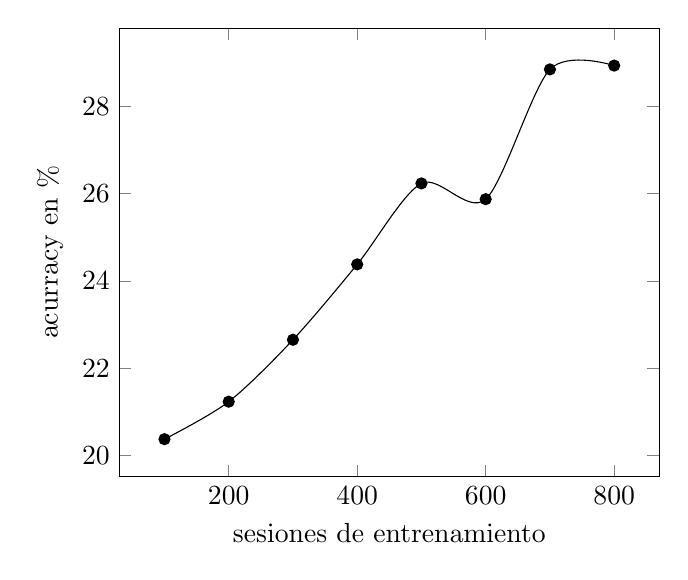
\begin{tikzpicture}
		\begin{axis}[
		xlabel=$\mbox{sesiones de entrenamiento}$,
		ylabel=$\mbox{acurracy en \%}$]
		\addplot[smooth,mark=*,black] plot coordinates {
			(100,  20.3715239154616)
			(200,  21.2302878598247)
			(300,  22.6490224129709)
			(400,  24.3752086811352)
			(500,  26.2308617234469)
			(600,  25.8692564745196)
			(700,  28.8423315814619)
			(800,  28.929431438127)
		};
		\end{axis}
		\end{tikzpicture}
		\caption{Experimento con secuencias de largo variable inferiore y 1000 sesiones}
		\label{fig:sim}
	\end{figure}
	
	El modelo sigue siendo válido al ir aumentando el volumen de datos bajo las mismas circunstancias. Incluso para ambos experimentos anteriores podemos sacar la relación que nuestro modelo posee una tasa de error de $\pm4\%$ al aumentar $100$ veces con respecto a la primera iteración de este escenario cuando se usa la  mayor cantidad de sesiones de entrenamiento posible.


	Otra particularidad que ha demostrado el modelo gracias a las propiedades de compresibilidad expuestas por  \emph{Lempel} \& \emph{Ziv}\cite{ZivLempel1977} es la minimización de niveles requeridos aún cuando la cantidad de nodos va creciendo.
	
	
	
	
	\begin{figure}[h] 
		\centering
			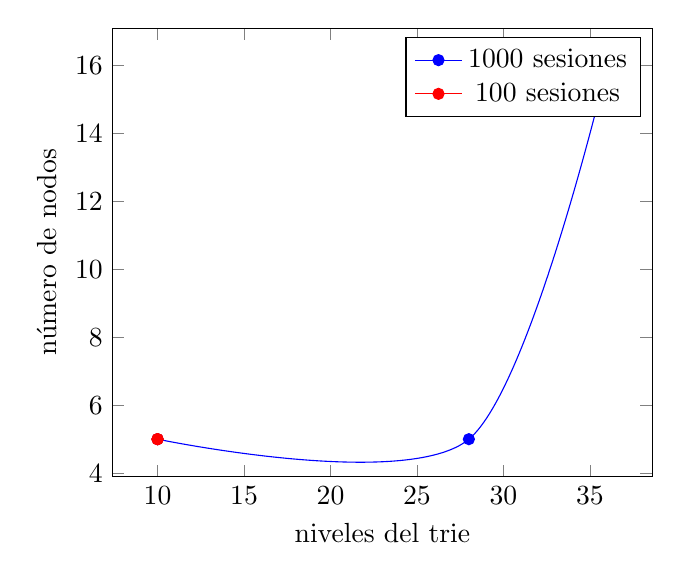
\begin{tikzpicture}
			\begin{axis}[
			xlabel=$\mbox{niveles del trie}$,
			ylabel=$\mbox{número de nodos}$]
			\addplot[smooth,mark=*,blue] plot coordinates {
				( 10 , 5 )
				( 28 , 5)
				( 36 , 16)
			};
			\addlegendentry{ 1000 sesiones }
			\addplot[smooth,mark=*,red] plot coordinates {
				( 10,5 )
				( 10,5 )
				( 10,5 )
			};
			\addlegendentry{ 100 sesiones }
			\end{axis}
			\end{tikzpicture}
		\caption{Gráfico comparativo para mismos niveles distinta cantidad de nodos.}
		\label{fig:sim}
	\end{figure}
	
	


	Como podemos ver en el comportamiento de inicio del modelo el criterio de partida en el escenario descrito es compartido por ambos experimentos.

	También dado a que no es uno de los escenarios más favorables para nuestro modelo predictivo, podríamos tener un diferencial en los tiempos de construcción del \emph{trie} respecto a la cantidad de nodos necesarios para el entrenamiento, 

	\begin{figure}[h] 
	\centering
	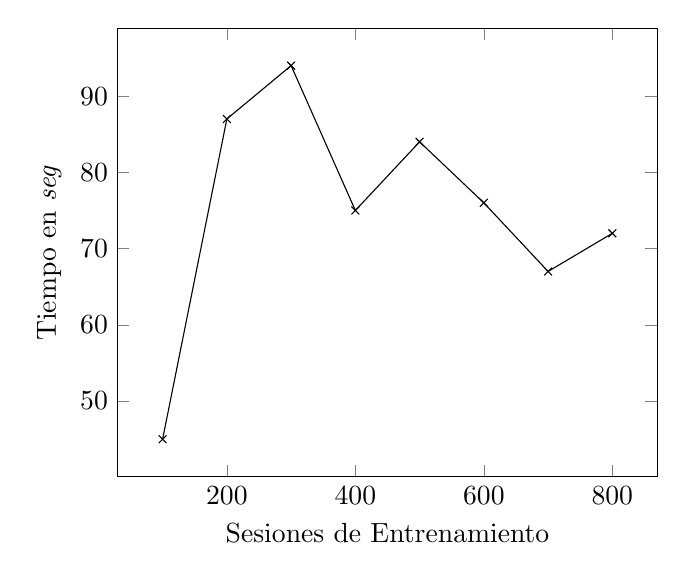
\begin{tikzpicture}
	\begin{axis}[
		xlabel= Sesiones de Entrenamiento ,
		ylabel= Tiempo en \emph{seg} ]
	\addplot[color=black,mark=x] coordinates {
			(100, 45 )
			(200, 87 )
			(300, 94 )
			(400, 75 )
			(500, 84 )
			(600, 76 )
			(700, 67)
			(800, 72 )
	};
	\end{axis}
	\end{tikzpicture}
		\caption{Gráfico de tiempo de construcción vs sesiones de entrenamiento}
	  \label{fig:sim}
	 \end{figure}	
	
	Como podemos ver en el gráfico anterior podemos buscar un dataset óptimo el cual puede encontrarse dentro del intervalo $ [ 300,400 ]$ sesiones de usuario, equivalente a la mejores resultados de \emph{Accurracy} y menor cantidad de secuencias de entrenamiento.


	\item \label{exp3}	
	\textbf{Sesiones con tamaño de secuencia constante}
	En este experimentos queremos lograr el mismo comportamiento que tuvimos en el experimento [\ref{exp1}]. Haciendo un filtrado simple de los \emph{webaccess log } que hemos estado analizando podemos llegar a mejores valores que las predicciones de resultado aleatorio.





	\begin{figure}[t] 
		\centering
			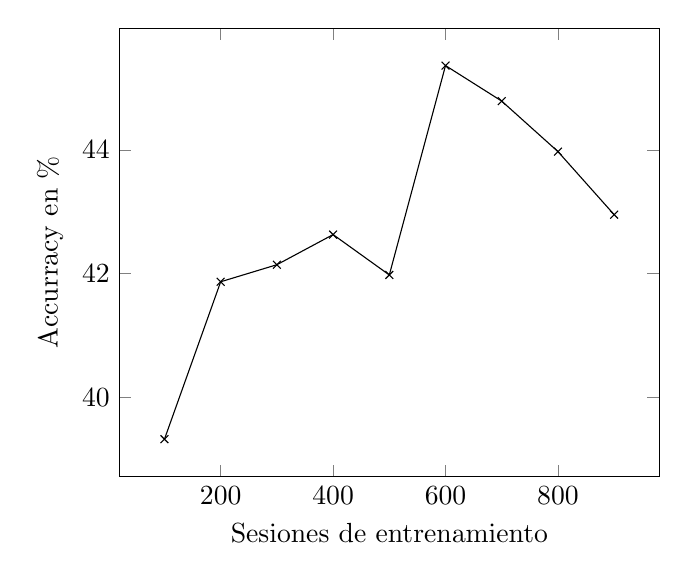
\begin{tikzpicture}
			\begin{axis}[
			xlabel=Sesiones de entrenamiento,
			ylabel=Accurracy en \% ]
			\addplot[color=black,mark=x] coordinates {
				(100, 39.3259176863181 )
				(200, 41.8698372966207 )
				(300, 42.1454458750596 )
				(400, 42.6323038397328 )
				(500, 41.9799599198396 )
				(600, 45.3634085213033 )
				(700, 44.7892976588628)
				(800, 43.9736180904522 )
				(900, 42.9539842873176 )
			};
			\end{axis}
			\end{tikzpicture}
		\caption{Gráfico de Accuracy vs sesiones de largo constante}
		\label{fig:sim}
	\end{figure}


\begin{table}[h] \label{my-label}
	\centering
	\resizebox{1\textwidth}{!}{
	\begin{tabular}{ccccc}
		\textbf{pruebas}     & \textbf{entrenamiento} & \textbf{accuracy}    & \textbf{nodos}       & \textbf{niveles}     \\
		800                  & 100                    & 0,203715239154616    & 150                  & 5                    \\
		700                  & 200                    & 0,212302878598247    & 150                  & 5                    \\
		600                  & 300                    & 0,226490224129709    & 300                  & 16                   \\
		500                  & 400                    & 0,243752086811352    & 1005                 & 48                   \\
		400                  & 500                    & 0,262308617234469    & 1005                 & 48                   \\
		300                  & 600                    & 0,258692564745196    & 1015                 & 48                   \\
		200                  & 700                    & 0,288423315814619    & 1023                 & 48                   \\
		100                  & 800                    & 0,28829431438127     & 1023                 & 48                   \\
		\multicolumn{1}{l}{} & \multicolumn{1}{l}{}   & \multicolumn{1}{l}{} & \multicolumn{1}{l}{} & \multicolumn{1}{l}{}
	\end{tabular}
	}
		\caption{Tabla resumen de experimento 3}
\end{table}

	
\begin{table}[]
	\centering \label{freq:exp3}
	\resizebox{1\textwidth}{!}{
	\begin{tabular}{lccccccccccccccccc}
		\textbf{símbolo}    & A   & B    & C   & D   & E   & F    & G   & H   & I   & J    & K   & L   & M   & N    & O  & P  & Q  \\
		\textbf{frecuencia} & 861 & 1502 & 509 & 412 & 557 & 1163 & 557 & 626 & 272 & 2252 & 399 & 703 & 301 & 1889 & 67 & 57 & 98
	\end{tabular}
	}
		\caption{Frecuencia de símbolos para experimentos con sesiones de largo constante.}	
	
\end{table}	
	
	
	La cantidad total de sesiones usadas fueron $1.000$ y las cuales como en el gráfico anterior se señala a mayor cantidad entrenamiento existe al menos un punto de la curva que se vuelve un máximo.


	Seguido a esto podemos ver el tiempo de construcción del \emph{trie} que nuestro modelo demora en generar:
	
	
	
	\begin{figure}[h] 
		\centering
		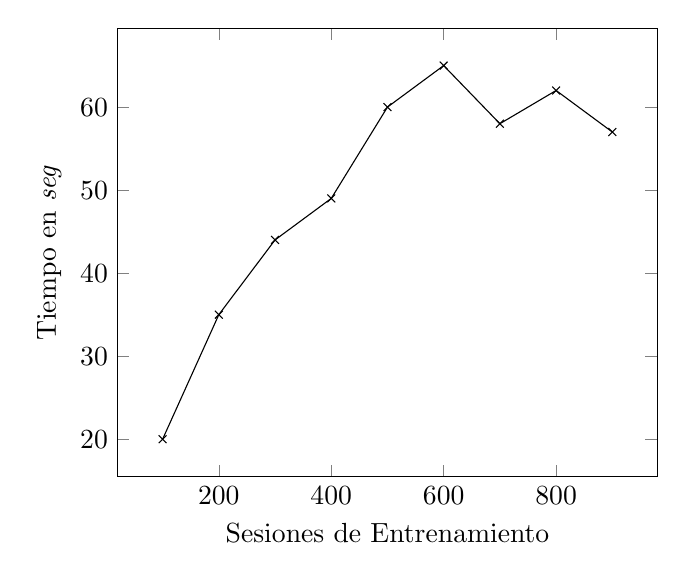
\begin{tikzpicture}
		\begin{axis}[
		xlabel= Sesiones de Entrenamiento ,
		ylabel=Tiempo en \emph{seg} ]
		\addplot[color=black,mark=x] coordinates {
			(100, 20)
			(200, 35)
			(300, 44)
			(400, 49)
			(500, 60)
			(600, 65)
			(700, 58)
			(800, 62)
			(900, 57 )
		};
		\end{axis}
		\end{tikzpicture}
		\caption{Gráfico de Tiempo vs sesiones de largo constante}
		\label{fig:sim}
	\end{figure}
	
	

	Al igual que en el gráfico anterior podemos ver que existe al menos una mínima cantidad sesiones las cuales generar un rendimiento sobre las evaluaciones a realizar. 
	

	\item \label{exp4} \textbf{Secuencias de accesos con limite inferior 100 símbolos }
	Este experimento busca validar las condiciones necesarias que debe tener una secuencia de entrada para que el algoritmo \texttt{LDC} pueda optimizar al momento de ser construido para una predicción \emph{online}, dado esto utilizaremos sesiones largas que entreguen redundancia en los accesos que permita al modelo de navegación ser más comprimido sin perder una métrica considerable para funcionar, según lo anterior realizamos las siguientes particiones de data que cumplen en el siguiente ciclo. 
	
	\begin{figure}[h] 
		\centering
		\resizebox{.7\textwidth}{!}{
		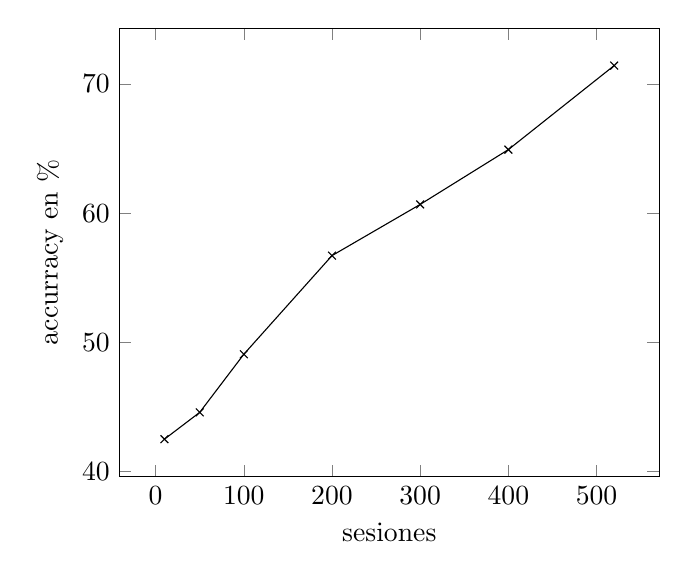
\begin{tikzpicture}
		\begin{axis}[
			xlabel= sesiones,
			ylabel=accurracy en \% ]
		\addplot[color=black,mark=x] coordinates {
			(10 ,  42.5190839694656 )
			(50 ,  44.595041322314 )
	 		(100 , 49.089861751152 )
	 		(200 , 56.7230538922155 )
	 		(300 , 60.6837606837608 )
	 		(400 , 64.9253731343282 )
	 		(520 , 71.4285714285715 )			
		};
		\end{axis}
		\end{tikzpicture}
		}
		\caption{Gráfico de Accuracy para sesiones mayores de 100 símbolos}
		\label{fig:sim}
	\end{figure}
	
	
	Sean la sesiones de entrenamiento de tamaño $T$, con un valor  $T(100) = 49 \% $ sobre un set de evaluación $E(100) = 900 \mbox{ sesiones}$ , nuestro modelo propuesto al igual que en el experimento \ref{exp1}, entrega un punto mínimo el cual al menos da un $50\%$ de acierto sobre el total de $535$ sesiones de usuarios, con una secuencia mínima de $100$ símbolos. Planteado de otra forma, sólo con el $20\%$ del total de datos de entrenamiento nuestro motor de predicción ya alcanza un \emph{Accurracy} que es mucho mejor que un predictor aleatorio sobre el alfabeto del experimento. Siendo este valor bastante optimista acorde a los puntos óptimos del predictor que use la menor cantidad de recursos.
	
	
	\begin{figure}[h] \label{fig:sim}
	\centering
		\resizebox{.7\textwidth}{!}{
		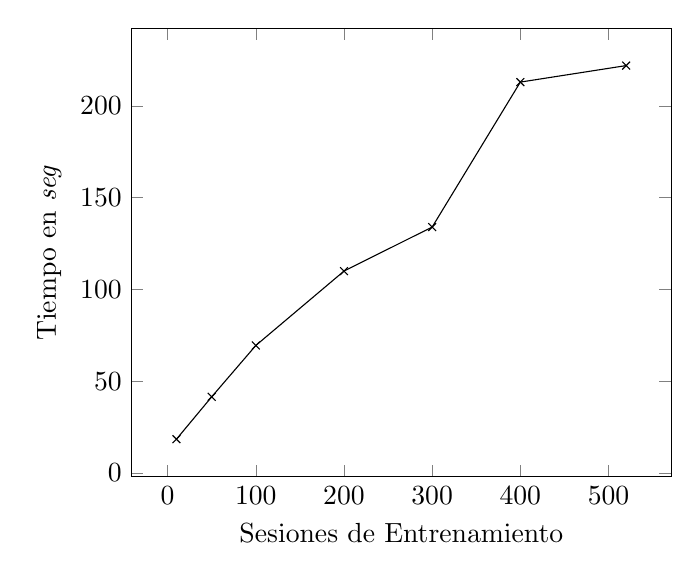
\begin{tikzpicture}
		\begin{axis}[
		xlabel= Sesiones de Entrenamiento ,
		ylabel=Tiempo en \emph{seg} ]
		\addplot[color=black,mark=x] coordinates {
			(10 ,  18.4)
			(50 ,  41.5)
			(100 , 69.46)
			(200 , 110)
			(300 , 134)
			(400 , 213)
			(520 , 222)	
		};
		\end{axis}
		\end{tikzpicture}
		}
		\caption{Gráfico de tiempo vs sesiones de entrenamiento\\ para sesiones mayores de 100 símbolos}
		
	\end{figure}


\begin{table}[h]
	\centering
	\caption{Tabla resumen experimento 4}
	\label{my-label}
	\begin{tabular}{ccccc}
		\textbf{pruebas} & \textbf{entrenamiento} & \textbf{accuracy} & \textbf{nodos} & \textbf{niveles} \\
		990              & 10                     & 0,21422649140546  & 38             & 5                \\
		950              & 50                     & 0,3104531085353   & 95             & 5                \\
		900              & 100                    & 0,393259176863181 & 132            & 5                \\
		800              & 200                    & 0,418698372966207 & 181            & 5                \\
		700              & 300                    & 0,421454458750596 & 208            & 5                \\
		600              & 400                    & 0,426323038397328 & 241            & 5                \\
		500              & 500                    & 0,419799599198396 & 264            & 5                \\
		400              & 600                    & 0,453634085213033 & 288            & 5                \\
		300              & 700                    & 0,407892976588628 & 308            & 5                \\
		200              & 800                    & 0,439736180904522 & 326            & 5                \\
		100              & 900                    & 0,429539842873176 & 349            & 5               
	\end{tabular}
\end{table}

\begin{table}[]
	\centering

	\label{my-label}
	\resizebox{0.9\textwidth}{!}{
	\begin{tabular}{lccccccccccccccccc}
		\textbf{símbolo}    & A    & B    & C   & D   & E   & F   & G   & H    & I   & J   & K   & L   & M   & N   & O   & P  & Q  \\
		\textbf{frecuencia} & 2162 & 1044 & 269 & 757 & 225 & 815 & 681 & 1207 & 370 & 278 & 233 & 453 & 502 & 860 & 102 & 10 & 32
	\end{tabular}
	}
	\caption{Tabla resumen de simbolos y frecuencia para experimento 4}
\end{table}

	Congruente con lo anterior podemos ver que sin tener un margen de error superior a la porción de datos seleccionado logramos un latencia de consulta predictiva en línea de alrededor de 70 \emph{seg}, el cual para ser implementado y consumido como ya se había mencionado antes como un algoritmo predictivo como servicio \texttt{REST}, esta dentro del promedio aceptable.

	\begin{figure}[h] 
		\centering
		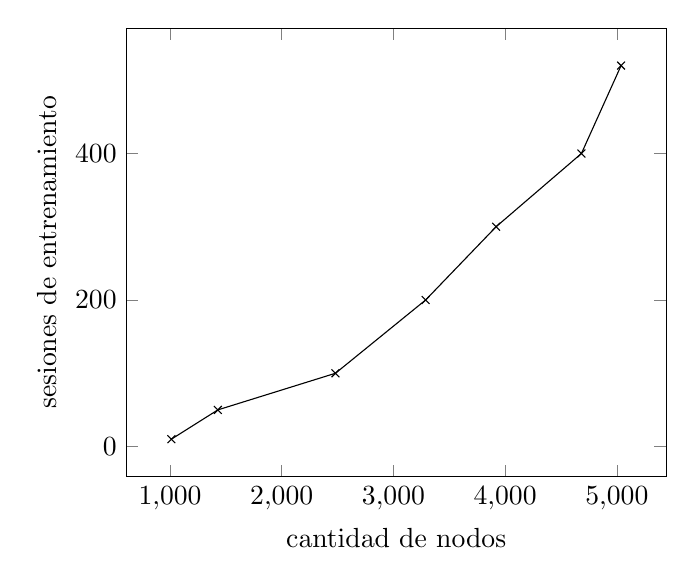
\begin{tikzpicture}
		\begin{axis}[
			xlabel= cantidad de nodos,
			ylabel= sesiones de entrenamiento  ]
		\addplot[color=black,mark=x] coordinates {
			(1012,10 )
			(1428,50 )
			(2481,100 )
			(3288,200 )
			(3919,300 )
			(4683,400 )
			(5038,520 )	
		};
		\end{axis}
		\end{tikzpicture}	
		\caption{Gráfico de cantidad de nodos vs sesiones de entrenamiento para sesiones mayores de 100 símbolos}
	  \label{fig:sim}
	\end{figure}


	Otro de los puntos  considerado aceptable, es que dado un set de entrenamiento $T(100)$, solo necesitaremos menos de la mitad de nodos que se requieren para llegar a un valor de predicción bueno, a diferencia de una partición de entrenamiento que requiere más del $90\%$ de nodos del total del set de datos.\\
	

	
	\begin{figure}[h] 
		\centering
			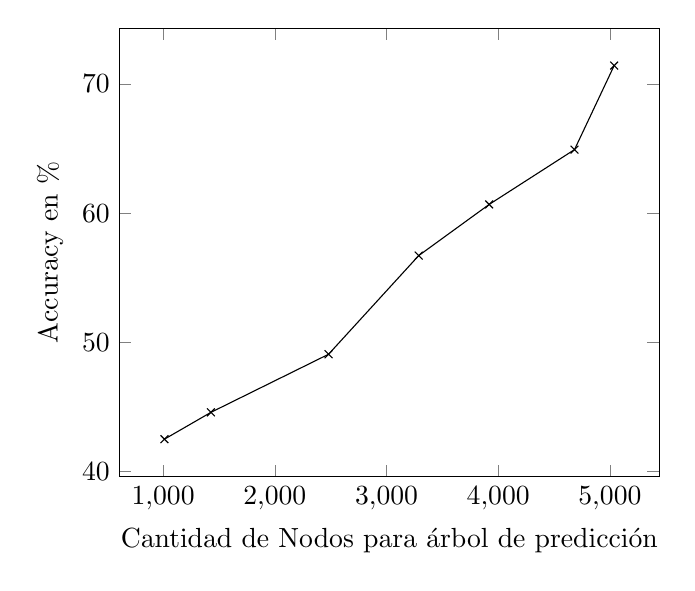
\begin{tikzpicture}
			\begin{axis}[
			xlabel=Cantidad de Nodos para árbol de predicción,
			ylabel=Accuracy en \%  ]
			\addplot[color=black,mark=x] coordinates {
				(1012,42.5190839694656 )
				(1428,44.595041322314 )
				(2481,49.089861751152 )
				(3288,56.7230538922155 )
				(3919,60.6837606837608 )
				(4683,64.9253731343282 )
				(5038,71.4285714285715 )	
			};	
			\end{axis}
			\end{tikzpicture}	
			\caption{Gráfico de cantidad de nodos vs Accuracy para sesiones mayor de 100 símbolos}
		\label{fig:sim}
	\end{figure}



	Finalmente podemos señalar que la tasa de \emph{Accuracy}, aún  subiendo al doble la cantidad de nodos para construir un \emph{trie} de \texttt{LZ78}, con mayor información  para predecir alcanza un rendimiento aceptable respecto de la compresión realizada. De todas maneras también se cumple que la cantidad de nodos del entrenamiento es directamente proporcional a la métrica seleccionada.


	\item \label{exp5}	
	\textbf{Sesiones con menos de 5 \emph{webaccess} para generar el \emph{trie}}
		Hacemos una validación cruzada para una muestra de data de 906130 sesiones de usuarios para probar como se comporta con {cross validation}.
	
	
	\begin{table}[tb]
		\centering
		\label{my-label}
				\resizebox{0.9\textwidth}{!}{
		\begin{tabular}{ccccc}
			\textbf{pruebas} & \textbf{entrenamiento} & \textbf{accuracy} & \textbf{nodos} & \textbf{niveles} \\
			990              & 10                     & 0,425190839694656 & 38             & 5                \\
			950              & 50                     & 0,44595041322314  & 95             & 5                \\
			900              & 100                    & 0,49089861751152  & 132            & 5                \\
			800              & 200                    & 0,567230538922155 & 181            & 5                \\
			700              & 300                    & 0,606837606837608 & 208            & 5                \\
			600              & 400                    & 0,649253731343282 & 241            & 5                \\
			500              & 520                    & 0,714285714285715 & 264            & 5               
		\end{tabular}
	}
			\caption{Tabla resumen experimento 6}
	\end{table}
	
	
	
	
	\begin{table}[tb]
		\centering
		\caption{Tabla resumen para sesiones mayores de 100000 sesiones}
		\label{my-label}
		\resizebox{.8\textwidth}{!}{
		\begin{tabular}{ccccc}
			\textbf{pruebas} & \textbf{entrenamiento}  & \textbf{accuracy} & \textbf{nodos} & \textbf{niveles} \\
			990              & 100                     & 0,299674371114825  & 61            & 4               \\
			950              & 200                     & 0,449237667712101  & 108           & 5               \\
			900              & 1000                    & 0,56519572924979   & 242           & 5               \\
			800              & 2500                    & 0,689237667712101  & 336           & 5               

		\end{tabular}
		}
	\end{table}
	
	
	
	\begin{figure}[h] 
		\centering
			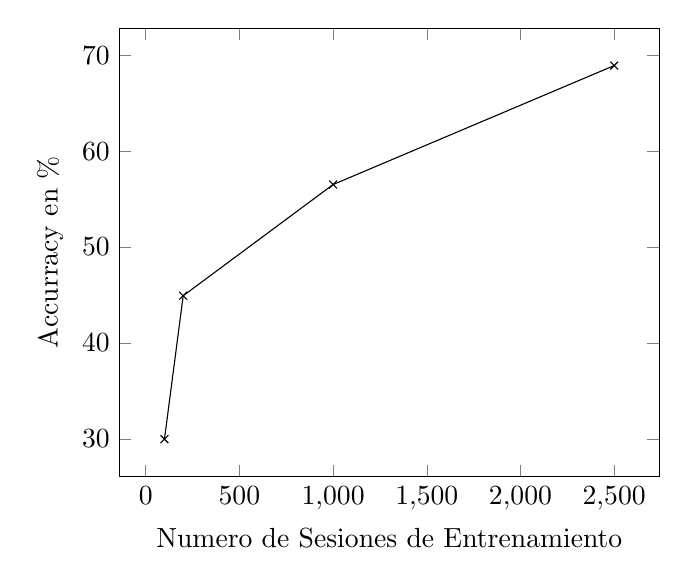
\begin{tikzpicture}
			\begin{axis}[
			xlabel= Numero de Sesiones de Entrenamiento,
			ylabel=Accurracy en \% ]
			\addplot[color=black,mark=x] coordinates {
				(100, 29.9674371114825)
				(200, 44.9237667712101)
				(1000, 56.519572924979)
				(2500, 68.9237667712101)	
			};
			\end{axis}
			\end{tikzpicture}
		\caption{Gráfico de Accuracy vs sesiones de entrenamiento para una cota superior de 5 símbolos}
		\label{fig:sim}
	\end{figure}
	
	\begin{table}[]
		\centering

		\label{my-label}
		\resizebox{1\textwidth}{!}{
		\begin{tabular}{lccccccccccccccccc}
			\textbf{símbolo}                                                                  & A                         & B                         & C                         & D                         & E                        & F                         & G                        & H                         & I                         & J                        & K                        & L                         & M                         & N                         & O                        & P                       & Q                       \\
			\textbf{\begin{tabular}[c]{@{}l@{}}frecuencia \\ 1000 sesiones\end{tabular}}      & 31086                     & 14262                     & 5483                      & 15458                     & 12713                    & 7717                      & 8255                     & 4155                      & 2381                      & 9697                     & 1974                     & 9584                      & 1871                      & 12795                     & 3935                     & 11735                   & 506                     \\
			\textbf{\begin{tabular}[c]{@{}l@{}}frecuencia \\ 100.000\\ sesiones\end{tabular}} & \multicolumn{1}{l}{43173} & \multicolumn{1}{l}{20251} & \multicolumn{1}{l}{15093} & \multicolumn{1}{l}{12790} & \multicolumn{1}{l}{1458} & \multicolumn{1}{l}{26517} & \multicolumn{1}{l}{4154} & \multicolumn{1}{l}{14517} & \multicolumn{1}{l}{12262} & \multicolumn{1}{l}{4163} & \multicolumn{1}{l}{4658} & \multicolumn{1}{l}{13180} & \multicolumn{1}{l}{14021} & \multicolumn{1}{l}{15779} & \multicolumn{1}{l}{2498} & \multicolumn{1}{l}{125} & \multicolumn{1}{l}{559}
		\end{tabular}
		}
		\caption{Tabla de frecuencia de símbolos para $1.000$ sesiones y $100.000$ }
	\end{table}
	
		
	
	
	\item \label{exp6} 
	\textbf{Detección de Ruido en secuencias de acceso}
	
	Al modelar una navegación de usuario mediante un \emph{trie} basado en un algoritmo como \texttt{LZ78}, adoptamos un enfoque basado en la frecuencia por lo cual si realizamos experimentos para poder encontrar ruido veremos que que son secuencias de acceso comunes y estas no dan relevancia o aportan a la exactitud ó precisión del algoritmo.
	
	Sea la secuencia $\{A,A,A,A,A,A,A,A,A,A,A,A \}$ a la cual llamaremos secuencia $R$, si $A$ es representado por el \emph{home} ó página de inicio, esto da a interpretación que existe un usuario en su sesión $R$ que se encuentra accediendo constantemente a esta sección. Podemos señalar que esta es una sesión ruidosa si:
	
	\begin{equation}
		P( x | AAAAAAA)= A ,	
	\end{equation} pero siendo la sesión $R$ de tamaño = $12$, en el siguiente acceso tendremos una probabilidad equiprobable dentro de las secciones en nuestro alfabeto, la cual generará un probabilidad de éxito ''falso positivo''.
	
	En el siguiente experimento veremos como se comporta nuestro modelo dado entradas \emph{Ruidosas}. Además se mostrará como el árbol suele perder su balance a medida que va creciendo los niveles de altura. 
	
	
	
	Por otro lado teniendo la noción de como es el funcionamiento de un servidor \texttt{IIS}, y al ser una página con un gran número de visitas, podemos señalar que los datos proporcionados no son totalmente representativos de usuarios reales, ya que la web al bien indexada en los buscadores existen un cantidad indeterminada de \emph{Crawlers} ó \emph{Bots} que están constantemente generando accesos tanto para almacenar en caché páginas o generando accesos automatizados a ciertos secciones sin ser datos representativo. Dejamos como discusión que algoritmo se podría implementar para detección de estos patrones por las ramas que hemos generado para la detección de \emph{bots} o \emph{robots}.
	
	
	
	
	 
	
	%	\item  Dataset uniformes de largo acotado inferiormente y volumenes de alto tamaño.
\end{enumerate}








 



	% \begin{forest} 
	% 	[VP
	% 	[DP]
	% 	[V’
	% 	[V]
	% 	[DP]
	% 	]
	% 	]
	% \end{forest}



	% \begin{tikzpicture}[level/.style={sibling distance=60mm/#1}]
	% \node [circle,draw] (z){$n$}
	% child {node [circle,draw] (a) {$\frac{n}{2}$}
	% 	child {node [circle,draw] (b) {$\frac{n}{2^2}$}
	% 		child {node {$\vdots$}
	% 			child {node [circle,draw] (d) {$\frac{n}{2^k}$}}
	% 			child {node [circle,draw] (e) {$\frac{n}{2^k}$}}
	% 		} 
	% 		child {node {$\vdots$}}
	% 	}
	% 	child {node [circle,draw] (g) {$\frac{n}{2^2}$}
	% 		child {node {$\vdots$}}
	% 		child {node {$\vdots$}}
	% 	}
	% }
	% child {node [circle,draw] (j) {$\frac{n}{2}$}
	% 	child {node [circle,draw] (k) {$\frac{n}{2^2}$}
	% 		child {node {$\vdots$}}
	% 		child {node {$\vdots$}}
	% 	}
	% 	child {node [circle,draw] (l) {$\frac{n}{2^2}$}
	% 		child {node {$\vdots$}}
	% 		child {node (c){$\vdots$}
	% 			child {node [circle,draw] (o) {$\frac{n}{2^k}$}}
	% 			child {node [circle,draw] (p) {$\frac{n}{2^k}$}
	% 				child [grow=right] {node (q) {$=$} edge from parent[draw=none]
	% 					child [grow=right] {node (q) {$O_{k = \lg n}(n)$} edge from parent[draw=none]
	% 						child [grow=up] {node (r) {$\vdots$} edge from parent[draw=none]
	% 							child [grow=up] {node (s) {$O_2(n)$} edge from parent[draw=none]
	% 								child [grow=up] {node (t) {$O_1(n)$} edge from parent[draw=none]
	% 									child [grow=up] {node (u) {$O_0(n)$} edge from parent[draw=none]}
	% 								}
	% 							}
	% 						}
	% 						child [grow=down] {node (v) {$O(n \cdot \lg n)$}edge from parent[draw=none]}
	% 					}
	% 				}
	% 			}
	% 		}
	% 	}
	% };
	% \path (a) -- (j) node [midway] {+};
	% \path (b) -- (g) node [midway] {+};
	% \path (k) -- (l) node [midway] {+};
	% \path (k) -- (g) node [midway] {+};
	% \path (d) -- (e) node [midway] {+};
	% \path (o) -- (p) node [midway] {+};
	% \path (o) -- (e) node (x) [midway] {$\cdots$}
	% child [grow=down] {
	% 	node (y) {$O\left(\displaystyle\sum_{i = 0}^k 2^i \cdot \frac{n}{2^i}\right)$}
	% 	edge from parent[draw=none]
	% };
	% \path (q) -- (r) node [midway] {+};
	% \path (s) -- (r) node [midway] {+};
	% \path (s) -- (t) node [midway] {+};
	% \path (s) -- (l) node [midway] {=};
	% \path (t) -- (u) node [midway] {+};
	% \path (z) -- (u) node [midway] {=};
	% \path (j) -- (t) node [midway] {=};
	% \path (y) -- (x) node [midway] {$\Downarrow$};
	% \path (v) -- (y)
	% node (w) [midway] {$O\left(\displaystyle\sum_{i = 0}^k n\right) = O(k \cdot n)$};
	% \path (q) -- (v) node [midway] {=};
	% \path (e) -- (x) node [midway] {+};
	% \path (o) -- (x) node [midway] {+};
	% \path (y) -- (w) node [midway] {$=$};
	% \path (v) -- (w) node [midway] {$\Leftrightarrow$};
	% \path (r) -- (c) node [midway] {$\cdots$};
	% \end{tikzpicture}



%Las conclusiones son deducidas logicamen- te de los resultados obtenidos y de la interpretacionpresen- tada, ademas estan conectadas al marco teorico.
%Las conclusiones muestran el logro de los ob jetivos.
%Se presentan proyec- ciones validas y valio- sas a partir del traba- jo realizado.
%Se detallan claramen- te las limitaciones del traba jo realizado.




 


 
%%%%%%%%
%%%%%%%%


 

El orden de como se ingresan las sesiones afecta directamente proporcional a la construcción del modelo \emph{trie},  por lo cual es un factor  \emph{FIFO} al momento de crear, lo primero que lee es lo primero que entrena por lo cual se debiese tener un criterio para ordenar los \emph{webaccess} antes de poder pasarlos al entrenador, que implica antes de la construcción.

El modelo propuesto, básicamente es un compresor el cual no toma decisiones, una posible mejora sería implementar un árbol de decisiones con algún criterio para decidir que entrenar y que no, estos árboles pueden estar dentro del \emph{trie} para
poder elegir secuencias optimo acorde a los criterios históricos, así podría darse el caso de ser un compresor--predictor  \emph{mas inteligente}.



















\uncm
\uncm
\section{Conclusiones y Contribuciones}\label{ch:conlusion-contrib-all}

Aún cuando se presenta varios antecedentes, podemos decir que nuestro modelo ocupa bastante menos memoria pero esto va directamente relacionado el tamaño del \emph{trie} de predicción generado.

%
Aun cuando el \emph{trie} que representa totalmente el modelo de navegación del los usuarios de un sitio web, este no puede generalizar completamente el comportamiento estocástico de los usuarios y/o agentes que acceden a los recursos de \emph{MSNBC} o un cualquier web en general.

Una de las mayores ventajas de nuestro modelo es que al estar embebido en un servidor de Machine Learning, cada nuevo evento que ingresa para la siguiente nueva ejecución esta estará mejor preparado, podríamos decir que la recolección de data de cada evento en particular nos ayudaría a que nuestro modelo en futuros trabajos vaya aprendiendo mas y más precisamente.


A medida que la altura del árbol va creciendo este genera mayor demora en cuanto a la creación del \emph{trie}.
% Pero a mayor altura hay mayor precisión.

Hemos validado que hacer un modelo de navegación de usuarios es un perfecta implementación de un predictor usando un árbol de la familia de \emph{Lempel} \& \emph{Ziv}.

A nuestro modelo le es afectado secuencias de menor tamaño, por lo cual se debe trabajar para hacer un aprendizaje de que momento omitirlo o no. Estas sesiones de bajo número de secuencias genera un bajo porcentaje de \emph{accurracy}. 


% Cual es el minimo entrenamiento para lograr a Predecir ?

Hemos presentado un modelo liviano el cual puede ser utilizado para predecir secuencias de \emph{webaccess} en demanda.






%In this paper we studied the empirical performance of a number of prominent prediction algorithms. We focused on prediction settings that are more closely related to those required

%%%%%%%%% On Prediction Using Variable Order Markov Models

%$%%%%%%%%
%%n this paper we studied the empirical performance of a number of prominent prediction algorithms. We focused on prediction settings that are more closely related to those required


%On Prediction Using Variable Order Markov Models
%by machine learning practitioners dealing with discrete sequences.
%However, somewhat surprisingly, the best predictor under the log-loss is not the best classifier. On the contrary, the consistently best protein classifier is based on the mediocre lz-ms predictor! This algo- rithm is a simple modification of the well-known Lempel-Ziv-78 (lz78) prediction algorithm, which can capture VMMs with large contexts. The surprisingly good classification accuracy achieved by this algorithm may be of independent interest to protein analysis research and clearly deserves further investigatio 
% Genero toda las referencias para demostrar el uso de la bibliografía
% No es necesario que utilice este comando en su document
%
%Conclusion of this paper Gopalratnam Cook
%a

lz modelos eficazmente procesos secuenciales, y es extremadamente útil para la predicción de los procesos donde los eventos son dependientes de la historia evento anterior. Esto es debido a la capacidad del algoritmo para construir un modelo preciso de la fuente de los eventos que se generan, una característica heredada de su información de fondo teórico y el algoritmo de compresión de texto \texttt{LZ78}.
%
La eficacia del método para el aprendizaje de una medida de tiempo también se puede atribuir a hecho de que ALZ es un fuerte predictor secuencial. Los principios teóricos de sonido en el que ALZ se fundamenta también significan que ALZ es un universal Quiniela óptima, y se puede utilizar en una variedad de escenarios de predicción.
%conclusion lcoa
%

Dado que la mayoría de los predictores funcionan de 
manera offline, uno de los aporte de tener estar estructura de algoritmos como servicios es poder tener un motor de predicción en linea.



\section{Contribución de esta Tesis}


En este trabajo,  nuestra principal contribución es el desarrollo del primer servidor de predicción de secuencias discretas con funcionalidad online y \emph{offline} para secuencias de  sitios web. Adicionalmente nuestro modelo en conjunto \emph{PredictionIO}, es el primer servidor de Machine Learning usando un modelo de predicción con un algoritmo de \emph{Lossless Data Compression}. Hay varios temas propuestos en el que este trabajo pueda tener iteraciones  futuras de estas sistema. 



\newpage
\section{Trabajos Futuro}

Esta memoria forma parte del plan de continuidad en el postgrado de la Escuela de Ingeniería Informática y telecomunicaciones, por lo cual se desea profundizar este trabajo en las discusiones realizadas. Los temas deseados por abarcar:

\begin{itemize}

\item Crear un estudio comparativo con Modelos de \emph{Machine Learning} como (\emph{RNN}) Redes Neuronales, Reglas de Asociación, \emph{Deep Learning} y algoritmo de tipo \emph{Frequent Pattern Growth}.

\item Técnicas para mejorar el modelo de predicción 
\item Mejorar la implementación de \texttt{LZ78}, realizado con lenguaje funcional y objetos(\emph{Scala}) y hacer una comparación de rendimientos contra implementaciones clásicas en lenguajes de más bajo nivel (\texttt{C++}).


\item Crear técnicas como la usada por \emph{Claude}~\etal~\cite{Claude2014}, para crear representaciones eficientes en función de este modelo predictivo.


\item Investigar los factores teóricos y técnicos para poder mejorar la exactitud de la predicción.

\item Ambiciosamente a realizar un estudio comparativo para encontrar puntos en común de estas áreas de la ciencia de la computación, se desea crear un nuevo algoritmo basado en la familia de \lempelziv, el cual pueda tener un complemento para la selección de sesiones antes ser ingresadas en el modelo de navegación predictivo. 


	
\end{itemize}	















 








